\documentclass{statsmsc}

\title{Parameter Bias in ETAS Models under Short-Term Incompleteness:
A Bayesian Approach}
\author{Seojeong Hong}
\CID{06058915}
\supervisor{Zak Varty}
\date{\today}
\logoimg{}

% THIS IS WHERE NEW COMMANDS CAN BE DEFINED
\newcommand{\consta}{a}
\newcommand{\X}{X}
\newcommand{\EE}[1]{ \mathrm{E} [ #1 ] }
\newcommand{\inparenth}[1]{\left( #1 \right)}

\usepackage{amsmath}
\usepackage{booktabs}
\usepackage{graphicx}
\usepackage{xcolor}
\usepackage{hyperref}
\hypersetup{
  colorlinks,
  linkcolor={blue!50!black},
  citecolor={blue!50!black},
  urlcolor={blue!50!black}
}

\newcommand{\Dobs}{\mathcal{D}_{\mathrm{obs}}}
\newcommand{\Hobs}{\mathcal{H}^{\mathrm{obs}}}

\begin{document}

% Generates the Title Page
\maketitle

% Generates plagiarism declaration
\declarationname{Seojeong Hong}
\declarationdate{\today}
\declaration

\begin{acknowledgements}
% First-draft placeholder. Replace this text in the final report with an
% accurate account of supervisory, computational, and other contributions.
Acknowledgements will be completed for the final dissertation.
\end{acknowledgements}

\clearpage
\tableofcontents
\clearpage

%=================================================================
% VERY IMPORTANT
% This command switches from Roman to Arabic numbering for main part of report.
% Do not modify.
\mainmatter
%=================================================================

\begin{abstract}
Short-term aftershock incompleteness occurs when small earthquakes are missed during periods of intense seismic activity. Ignoring this observation process can bias inference for Epidemic-Type Aftershock Sequence (ETAS) models.
Although time-varying completeness corrections can improve parameter estimation, it remains unclear whether the resulting Bayesian credible
intervals achieve their nominal coverage across repeated catalogues.
This study evaluates the parameter recovery, interval calibration, and
predictive performance of a time-varying completeness correction. Naive ETAS,
which treats the observed catalogue as complete, is compared with a Plug-in
model that adjusts the likelihood using completeness parameters estimated
before ETAS fitting and subsequently held fixed. The models are evaluated
using 100 simulated incomplete catalogues and a held-out test period from the
2019 Ridgecrest earthquake sequence.
In the simulation study, the Plug-in correction substantially reduces
estimation error and improves the empirical coverage of 95\% credible
intervals for key triggering parameters, particularly productivity, magnitude
scaling, and the Omori offset. These improvements are not uniform across all
ETAS parameters. In the Ridgecrest analysis, the correction produces a modest
improvement in temporal predictive density and a predicted event-count median
closer to the observed total, but also yields a more dispersed count
distribution with a heavier upper tail. Overall, modelling short-term
incompleteness improves inference for several important ETAS parameters, while
its benefits for real-data prediction remain mixed.
\end{abstract}

\section{Introduction}

The Epidemic-Type Aftershock Sequence (ETAS) model represents an earthquake catalogue as a self-exciting point process that combines background seismicity with earthquake-triggered activity \citep{ogata1988}. In a self-exciting process, the occurrence of an earthquake temporarily increases the rate of subsequent earthquakes. Each event may therefore trigger direct aftershocks, which may themselves trigger further events, producing a branching sequence over multiple generations. ETAS models are used to characterise this triggering behaviour and to forecast future seismic activity \citep{mizrahi2021}. Reliable parameter estimation is important because the productivity parameters determine the expected number of triggered events and how this number varies with parent magnitude, while the modified Omori parameters determine the temporal concentration and decay of aftershock activity. Biased estimates may therefore distort both the scientific interpretation of earthquake triggering and forecasts of future seismicity.

ETAS models are typically fitted to earthquakes above a fixed baseline
magnitude threshold \(m_0\), under the assumption that the resulting catalogue
is complete. In contrast, the time-dependent magnitude of completeness
\(m_c(t)\) is the lowest magnitude above which earthquakes are considered
reliably detected at time \(t\). Immediately after a large earthquake,
overlapping seismic waveforms and elevated noise can reduce the detectability
of small aftershocks. Consequently, \(m_c(t)\) may temporarily rise above
\(m_0\), before gradually returning towards the baseline threshold as
aftershock activity decays \citep{omi2014,hainzl2016}. During periods when
\(m_c(t)>m_0\), some earthquakes included in the target magnitude range of the
ETAS model are therefore missing from the observed catalogue.

From a statistical perspective, earthquake detection is not independent of
the underlying seismicity process. The probability that an earthquake is
detected depends on its magnitude and on the time elapsed since a large
earthquake, and is lowest during the early period when the aftershock rate is
highest \citep{omi2014,hainzl2016}. In this study, an ETAS model that ignores
this time-varying observation process is referred to as Naive ETAS. Because
Naive ETAS treats the observed catalogue as complete above \(m_0\), it may
interpret the small number of recorded early aftershocks as a feature of the
seismicity process rather than as a detection failure. This can bias estimates
of the productivity and temporal-decay parameters
\citep{seif2017,naylor2023}, thereby distorting the inferred number, magnitude
dependence, and timing of triggered earthquakes. Such distortions may affect
both the scientific interpretation of aftershock sequences and the predictive
performance of the fitted model.

The problem is compounded by the ETAS branching structure. Because each
earthquake may act as a parent of subsequent events, a missed earthquake is
absent not only as an observed outcome but also as a possible source of later
triggering. Suppose that an observed mainshock \(A\) triggers an undetected
event \(B\), which then triggers an observed event \(C\). A model conditioned
only on the observed history sees \(A\) and \(C\), but cannot include the
contribution of \(B\) to the conditional intensity at the time of \(C\). It
must therefore explain \(C\) through the background rate or through triggering
by an observed event. Multiplying the observed-history intensity by a
detection probability can adjust the expected rate of detected events, but it cannot account for the additional triggering caused by undetected events.

Several approaches address short-term aftershock incompleteness. Empirical
detection models estimate time-varying detection functions from observed
magnitude distributions and incorporate them into ETAS estimation
\citep{omi2014}. Rate-dependent approaches link short-term changes in
catalogue completeness to the seismicity rate \citep{hainzl2016}. PETAI uses
an expectation--maximisation scheme to estimate detection and ETAS parameters
self-consistently and has been evaluated using synthetic catalogues and
pseudo-prospective forecasts \citep{mizrahi2021}. These studies provide strong
evidence that incompleteness affects parameter estimation and forecasting, but
they do not directly evaluate the repeated-sampling calibration of Bayesian
credible intervals.

Bayesian ETAS inference represents parameter uncertainty through a posterior
distribution. \citet{naylor2023} showed that short-term incompleteness can
substantially distort ETAS posteriors. More recently,
\citet{kamranzad2025} introduced a time-dependent correction for the reduced
detectability of small earthquakes after a large event. Their method derives
the detectable fraction of earthquakes from a log-linear completeness curve
and incorporates this fraction into the ETAS intensity and likelihood, thereby
adjusting the model-implied rate of observed earthquakes. In synthetic
examples, the corrected posterior distributions were closer to the true
data-generating parameter values than those obtained from standard ETAS, which
showed substantial displacement from the truth. The method was also applied
to three real earthquake sequences. This approach is useful because it can
account for time-varying incompleteness without explicitly reconstructing
undetected earthquakes, making it comparatively straightforward to incorporate
into ETAS inference. However, the completeness parameters are estimated before
ETAS fitting and then held fixed, so their estimation uncertainty is not
propagated into the ETAS posterior. Moreover, the synthetic analysis assessed
posterior recovery in selected scenarios rather than the empirical coverage of
credible intervals across repeated catalogues.
Improved parameter recovery does not necessarily imply reliable uncertainty
quantification or improved prediction for a real earthquake sequence. It
therefore remains necessary to evaluate both the empirical coverage of
Bayesian credible intervals across repeated catalogues and held-out predictive
performance. In this dissertation, predictive performance is assessed using
temporal log predictive density and event-count prediction. The correction
uses only the observed earthquake history and does not explicitly infer
undetected earthquakes or their triggering contributions.

Accordingly, this dissertation addresses two research questions:
\begin{description}
  \item[RQ1.] Under short-term catalogue incompleteness, to what extent does
  a Plug-in time-varying completeness correction improve ETAS parameter
  recovery and the empirical coverage of Bayesian credible intervals relative
  to Naive ETAS?
  \item[RQ2.] Does the same correction improve short-term predictive
  performance in the Ridgecrest sequence, as measured by temporal log
  predictive density and event-count prediction?
\end{description}

These questions are addressed through two main analyses. First, Naive ETAS
and the time-varying completeness correction proposed by
\citet{kamranzad2025}, implemented here as a Plug-in model, are fitted to the
same set of repeatedly simulated incomplete catalogues, enabling paired
comparisons between the two models. Posterior inference is performed using
MCMC, and parameter recovery and empirical coverage are compared across the
repeated catalogues. Second, temporal and event-count predictive performance
is evaluated over a fixed held-out period from the Ridgecrest sequence. The
contribution therefore lies in evaluating the inferential reliability and
predictive limitations of an existing completeness correction, rather than in
introducing a new physical model of catalogue completeness.

The remainder of the report is organised as follows. Section~\ref{sec:methods}
defines the temporal ETAS and observation models and presents the simulation
and Ridgecrest evaluation designs. Section~\ref{sec:results} reports parameter
recovery and interval calibration, followed by the Ridgecrest test-period
results. The Discussion relates these findings to previous incompleteness
methods, describes the limitations of the observed-history correction, and
identifies latent-event inference as a direction for future work.



\section{Methods}\label{sec:methods}
\subsection{Temporal ETAS model}\label{subsec:temporal_etas}

Let
\(\mathcal{H}_t=\{(t_i,m_i):t_i<t\}\) denote the observed earthquake history
before time \(t\), where \(t_i\) and \(m_i\) are the occurrence time and
observed magnitude of event \(i\), respectively. The conditional intensity
\(\lambda(t\mid\mathcal{H}_t,\theta)\) represents the instantaneous rate of
earthquake occurrence at time \(t\), given this history. In the temporal ETAS
model, the intensity is the sum of a constant background rate and triggering
contributions from all previous earthquakes:
\begin{equation}
\lambda(t\mid\mathcal{H}_t,\theta)
=
\mu+
\sum_{i:t_i<t}
K\,10^{\alpha(m_i-m_0)}
g(t-t_i;c,p),
\label{eq:etas}
\end{equation}
where
\[
g(u;c,p)
=
\frac{p-1}{c}
\left(1+\frac{u}{c}\right)^{-p},
\qquad u>0,
\]
is the normalised modified Omori temporal kernel. The parameter vector is
\(\theta=(\mu,K,\alpha,c,p)\). The background rate \(\mu\) determines the
expected number of events per unit time that are not attributed to previous
observed earthquakes. The productivity term
\(K10^{\alpha(m_i-m_0)}\) is the expected number of direct offspring triggered
by an event of magnitude \(m_i\). In particular, \(K\) is the expected direct
productivity of an event at the baseline magnitude \(m_0\), while \(\alpha\)
determines how rapidly productivity increases with parent magnitude. The
kernel \(g(u;c,p)\) distributes these offspring over elapsed time \(u\) after
the parent event. The parameter \(c\) controls the concentration of triggering
immediately after the parent event, while \(p\) controls the subsequent rate
of temporal decay. The model requires \(\mu,K>0\), \(\alpha\geq0\), \(c>0\),
and \(p>1\).

The point-process likelihood evaluates whether the conditional intensity
assigns high rates at the observed event times without implying an
unreasonably large number of events over the full observation window. It
therefore contains two components: the product of the intensities at the
observed event times and a penalty determined by the integrated intensity.
For an observation window \((T_1,T_2]\), the likelihood is
\[
L(\theta)
=
\left\{
\prod_{\substack{i\in\mathcal I\\T_1<t_i\leq T_2}}
\lambda(t_i\mid\mathcal H_{t_i},\theta)
\right\}
\exp\left\{
-\int_{T_1}^{T_2}
\lambda(t\mid\mathcal H_t,\theta)\,dt
\right\},
\]
where \(\mathcal I\) denotes the events treated as likelihood targets. Taking
logarithms gives
\begin{equation}
\ell(\theta)
=
\sum_{\substack{i\in\mathcal I\\T_1<t_i\leq T_2}}
\log\lambda(t_i\mid\mathcal H_{t_i},\theta)
-
\int_{T_1}^{T_2}
\lambda(t\mid\mathcal H_t,\theta)\,dt.
\label{eq:pp_likelihood}
\end{equation}
The first term rewards parameter values that assign high conditional
intensity at the observed event times. The second term is the model-implied
expected number of events over the observation window and penalises parameter
values that assign excessively high intensity throughout that window.

Conditional on event occurrence, magnitudes are modelled as independent marks
using the Gutenberg--Richter magnitude--frequency relation. This empirical
relation states that the expected number of earthquakes with magnitude at
least \(m\) satisfies
\[
\log_{10}N(M\geq m)=a-bm,
\]
where \(a\) controls the overall level of seismic activity and \(b\) controls
how rapidly earthquake frequency decreases with increasing magnitude.
Conditioning on earthquakes above the baseline magnitude \(m_0\) gives
\[
\Pr(M\geq m\mid M\geq m_0)
=
\frac{10^{a-bm}}{10^{a-bm_0}}
=
10^{-b(m-m_0)},
\qquad m\geq m_0.
\]
Equivalently, \(M-m_0\) follows an exponential distribution with rate
\(\beta=b\log 10\).

The branching ratio \(n\) is the expected number of direct offspring per
earthquake, averaged over the distribution of parent magnitudes. It provides a
summary of the overall level of earthquake triggering and is reported
alongside \(K\) and \(\alpha\), because different combinations of these two
parameters can imply similar overall productivity.

Because the temporal kernel \(g(u;c,p)\) integrates to one, the productivity
term \(K10^{\alpha(m-m_0)}\) gives the expected number of direct offspring
triggered by an earthquake of magnitude \(m\). Averaging this quantity over
the Gutenberg--Richter magnitude distribution gives the infinite-window
branching ratio

\[
n
=
K\frac{b}{b-\alpha},
\qquad \alpha<b.
\]

\subsection{Short-term incompleteness and inference}
\label{subsec:loglinear_incompleteness}

The observation model follows the empirical log-linear completeness recovery
used by \citet{helmstetter2006} and the Bayesian correction of
\citet{kamranzad2025}. Following a large earthquake, the magnitude threshold
above which events are reliably detected is initially elevated because small
aftershocks may be obscured during the period of highest seismic activity. The
log-linear model represents the subsequent recovery in detectability by
allowing this threshold to decline linearly with the logarithm of elapsed time
since the mainshock. It is used here as a deliberately simplified description
of short-term incompleteness rather than as a complete physical model of
seismic-network detection. Its two-parameter form provides a common and
controllable observation mechanism that can be applied across simulated
catalogues, allowing the inferential consequences of incompleteness to be
evaluated under a known data-generating process.

Following a designated mainshock at time \(t_m\) with observed magnitude
\(m_m\), the effective completeness magnitude is

\begin{equation}
m_c(t)
=
\max\left\{
m_0,\,
m_m-G-H\log_{10}(t-t_m)
\right\},
\qquad t>t_m.
\label{eq:mct}
\end{equation}

Elapsed time \(t-t_m\) is measured in days. Specifying the unit is necessary
because changing the time unit inside the logarithm changes the numerical
interpretation of the intercept \(G\). The parameter \(G\) controls the
initial level of the non-baseline completeness threshold, while \(H>0\)
controls the rate at which it declines with \(\log_{10}(t-t_m)\). The maximum
with \(m_0\) ensures that the completeness threshold does not fall below the
baseline magnitude used for ETAS analysis.

The observation model is defined relative to a single designated mainshock.
It therefore represents one temporary increase in the completeness threshold
and does not allow subsequent large earthquakes to initiate additional or
overlapping completeness-recovery curves. The model should consequently be
interpreted as a single-mainshock approximation rather than as a general
observation model for multiple overlapping sequences. Its specific
implementation in the synthetic and Ridgecrest analyses is described in
Sections~\ref{subsec:simulation_design} and
\ref{subsec:ridgecrest_design}, respectively.

Under the Gutenberg--Richter magnitude model, the probability that an
earthquake above \(m_0\) also exceeds the time-dependent completeness
threshold is

\[
\psi(t;G,H)
=
\Pr\{M\geq m_c(t)\mid M\geq m_0\}
=
10^{-b\{m_c(t)-m_0\}}.
\]

In the synthetic experiment, incompleteness is imposed as a hard threshold:
an event is retained if \(m_i\geq m_c(t_i)\). After averaging over the
Gutenberg--Richter magnitude distribution, \(\psi(t;G,H)\) is therefore the
expected fraction of events above \(m_0\) that are detectable at time \(t\).

The Gutenberg--Richter parameter is fixed at \(b=1\), a commonly used
reference value, in both the synthetic and Ridgecrest analyses. Estimating
\(b\) jointly with \(G\) and \(H\) would introduce additional dependence
between the magnitude distribution and the completeness curve, because
\(b\), \(G\), and \(H\) all affect the observed magnitude pattern and the
detectable fraction \(\psi(t;G,H)\). Fixing \(b\) keeps the magnitude model
consistent across the two analyses and allows the study to focus on the
effect of the time-varying completeness correction. The results are therefore
conditional on \(b=1\); sensitivity to estimating or varying \(b\) is not
assessed.

The completeness parameters \(G\) and \(H\) are estimated from observed
post-mainshock magnitudes, conditional on their occurrence times. Under the
Gutenberg--Richter model, \(M-m_0\) is exponentially distributed with rate
\(\beta=b\log 10\). Conditional on an event exceeding the higher threshold
\(m_c(t_i;G,H)\), the memoryless property of the exponential distribution
therefore gives

\[
M-m_c(t_i;G,H)
\mid M\geq m_c(t_i;G,H)
\sim \operatorname{Exponential}(\beta).
\]

Consequently, for candidate values of \(G\) and \(H\) satisfying
\(m_i\geq m_c(t_i;G,H)\) for every included event, the conditional
log-likelihood is

\begin{equation}
\ell_{\mathrm{mag}}(G,H)
=
\sum_{i:t_i>t_m}
\left[
\log\beta-\beta\{m_i-m_c(t_i;G,H)\}
\right],
\label{eq:gh_likelihood}
\end{equation}

and is \(-\infty\) otherwise. Because increasing \(m_c(t_i;G,H)\) reduces the
exceedance \(m_i-m_c(t_i;G,H)\), the likelihood favours a completeness curve
that lies as high as possible while remaining below every included observed
magnitude. The temporal pattern of the lower magnitude envelope identifies
the intercept \(G\) and decay parameter \(H\), subject to the specified
constraints. The Plug-in estimates are

\[
(\widehat G,\widehat H)
=
\arg\max_{3\leq G\leq7,\;0.2\leq H\leq1.5}
\ell_{\mathrm{mag}}(G,H).
\]

These bounds are specified before fitting and applied to every catalogue. The
estimation uses the observed magnitudes conditional on their occurrence times,
but does not use the ETAS event-time likelihood. Thus, \(G\) and \(H\) are
estimated before ETAS fitting and subsequently treated as fixed.

The Naive model fits Equation~\eqref{eq:pp_likelihood} directly to the
incomplete catalogue and therefore treats the observed history as complete
above \(m_0\). Let
\(\mathcal H_t^{\mathrm{obs}}\subset\mathcal H_t\) denote the history of
recorded events before time \(t\). For the Plug-in model, thinning by the
time-dependent detectable fraction motivates the observed-event intensity

\begin{equation}
\lambda_{\mathrm{plug}}
(t\mid\mathcal H_t^{\mathrm{obs}},\theta)
=
\psi(t;\widehat G,\widehat H)
\left[
\mu+
\sum_{i:(t_i,m_i)\in\mathcal H_t^{\mathrm{obs}}}
K10^{\alpha(m_i-m_0)}
g(t-t_i;c,p)
\right].
\label{eq:plugin}
\end{equation}

To show how this correction affects ETAS inference, let the expression in
square brackets be denoted by
\(\lambda_{\mathrm{obs}}(t\mid\mathcal H_t^{\mathrm{obs}},\theta)\).
Substituting Equation~\eqref{eq:plugin} into the point-process log-likelihood
gives

\[
\ell_{\mathrm{plug}}(\theta)
=
\sum_{\substack{i\in\mathcal I\\T_1<t_i\leq T_2}}
\log\lambda_{\mathrm{obs}}
(t_i\mid\mathcal H_{t_i}^{\mathrm{obs}},\theta)
+
\sum_{\substack{i\in\mathcal I\\T_1<t_i\leq T_2}}
\log\psi(t_i;\widehat G,\widehat H)
-
\int_{T_1}^{T_2}
\psi(t;\widehat G,\widehat H)
\lambda_{\mathrm{obs}}
(t\mid\mathcal H_t^{\mathrm{obs}},\theta)\,dt.
\]

Conditional on \((\widehat G,\widehat H)\), the middle term does not vary with
the ETAS parameters \(\theta\). Relative to the Naive likelihood, the
correction therefore changes ETAS parameter estimation through the integrated
intensity, which now represents the model-implied expected number of detected,
rather than underlying, events. The posterior is proportional to
\(\exp\{\ell_{\mathrm{plug}}(\theta)\}p(\theta)\).

The triggering sum in Equation~\eqref{eq:plugin} contains recorded events
only. The Plug-in model therefore adjusts the expected rate of detected events
but does not infer unobserved earthquakes or include the additional triggering
caused by them. It is consequently an observed-history approximation rather
than a latent-event ETAS model.

\subsection{Synthetic experiment and posterior computation}
\label{subsec:simulation_design}

A total of \(R=100\) complete temporal ETAS catalogues are simulated over
\(0\)--\(1500\) days. Following \citet{morris2019}, the replication count was
selected to balance Monte Carlo precision against computational cost. If the
true coverage is 0.95, \(R=100\) gives a Monte Carlo standard error of
\[
\sqrt{\frac{0.95(1-0.95)}{100}}
=
0.022.
\]
The paired comparison requires 200 model fits, each using four MCMC chains.

The broad simulation design follows \citet{kamranzad2025}. The 500-day
pre-mainshock period provides a relatively quiet history from which the
background rate can be identified, while the 1000-day post-mainshock period
allows the triggered sequence to decay towards its background level. A
background rate of \(\mu=0.10\) events per day, Gutenberg--Richter parameter
\(b=1\), baseline magnitude \(m_0=2.5\), and a magnitude 6.5 mainshock at
day 500 provide a setting comparable to their synthetic experiments.

The remaining data-generating parameters are
\[
(K,\alpha,c,p)=(0.21,0.70,0.01,1.20).
\]
The productivity parameters are specified through a branching ratio of
\(n=0.70\), which is below the critical value \(n=1\) while retaining
multi-generation triggering. Under the normalised ETAS parameterisation,
\(b=1\), \(\alpha=0.70\), and \(n=0.70\) imply
\[
K=n\frac{b-\alpha}{b}=0.21.
\]
The values \(c=0.01\) days and \(p=1.20\) concentrate triggering shortly
after each parent event while retaining a decaying temporal tail. The
data-generating process is therefore subcritical, with a finite expected
cluster size, but contains pronounced early aftershock activity during which
short-term incompleteness can operate.

The magnitude 6.5 mainshock is inserted as an externally specified
conditioning event. It is included in the earthquake history and may trigger
subsequent events, but its own occurrence is excluded from the likelihood.
The seeded mainshock is also the only event specified to initiate the
temporary increase in the completeness threshold. Incomplete catalogues are
produced using Equation~\eqref{eq:mct} with \(G=4.5\) and \(H=0.75\). Each
replicate therefore provides a latent complete catalogue and its incomplete
observed counterpart. The complete catalogue is retained for simulation
diagnostics, whereas both Naive and Plug-in ETAS are fitted to the same
incomplete catalogue. This produces a paired comparison between the two
methods within each replicate.

Both models are fitted using the same ETAS priors:
\[
\begin{aligned}
\mu&\sim\operatorname{Gamma}(\text{shape}=0.5,\text{rate}=0.5),&
K&\sim\operatorname{Lognormal}(-1,1^2),\\
\alpha&\sim\operatorname{Uniform}(0.05,2),&
c&\sim\operatorname{Uniform}(0.001,0.2),&
p&\sim\operatorname{Uniform}(1.01,2.5).
\end{aligned}
\]
The prior specification is adapted from the broad ETAS.inlabru priors of
\citet{naylor2023} and is fixed independently of the data-generating parameter
values. The Gamma and lognormal priors enforce positivity for \(\mu\) and
\(K\). The bounded uniform priors define a common fitting domain for
\(\alpha\), \(c\), and \(p\), with the lower bound on \(p\) ensuring an
integrable temporal kernel. Applying the same priors to both models ensures
that posterior differences arise from their likelihoods rather than from
different prior assumptions.

The priors do not constrain the fitted process to be subcritical. Under the
assumed unbounded Gutenberg--Richter magnitude distribution, posterior draws
with \(\alpha\geq b\) have an unbounded infinite-window branching ratio.
These draws are retained so that potential instability in the fitted process
is not hidden by an additional prior restriction.

Posterior inference is performed using an adaptive random-walk Metropolis
algorithm. The positive parameters \(\mu\) and \(K\) are sampled on the log
scale, while the bounded parameters \(\alpha\), \(c\), and \(p\) are mapped
to the real line using logit transformations. The corresponding Jacobian is
included in the target density. Preliminary INLA/Laplace fits provide initial
values and proposal covariance matrices only. Their approximate posterior
draws are not included in the reported posterior summaries; the subsequent
MCMC target is determined solely by the likelihood and priors specified
above.

Four MCMC chains are run for 12,000 iterations each. The first 4,000
iterations of each chain are discarded as warm-up, and every fourth subsequent
draw is retained, giving 8,000 draws after combining the four chains. The
sampler jointly updates all five transformed ETAS parameters. During warm-up,
the proposal scale is adapted towards the conventional multivariate
random-walk Metropolis acceptance target of 0.234 and is then fixed for
posterior sampling \citep{roberts1997}.

Convergence is assessed separately for each ETAS parameter. The classical
Gelman--Rubin statistic \(\widehat R\) compares within-chain and between-chain
variation, with values close to one indicating that the chains have reached
similar distributions. Effective sample size measures the amount of
approximately independent posterior information after accounting for
autocorrelation. A fit passes the pre-specified convergence gate when every
parameter has \(\widehat R\leq1.05\) and a combined effective sample size of
at least 400. A failed fit is rerun using 24,000 iterations and 8,000 warm-up
iterations and must satisfy the same convergence criteria.

\subsection{Simulation evaluation}\label{subsec:evaluation}

Parameter recovery is evaluated using bias and root mean squared error
(RMSE). Bias measures systematic estimation error, whereas RMSE measures
overall error across simulated catalogues. For parameter \(k\), let
\(\theta_k^0\) denote the true value and \(\widetilde{\theta}_{kr}\) the
posterior median in replicate \(r\), where \(k=1,\ldots,5\),
\(r=1,\ldots,R\), and \(R=100\). Then
\[
\operatorname{Bias}_k
=
\frac{1}{R}\sum_{r=1}^{R}
(\widetilde{\theta}_{kr}-\theta_k^0),
\qquad
\operatorname{RMSE}_k
=
\left\{
\frac{1}{R}\sum_{r=1}^{R}
(\widetilde{\theta}_{kr}-\theta_k^0)^2
\right\}^{1/2}.
\]
Credible-interval calibration is evaluated using empirical coverage. For each
replicate, the equal-tailed 95\% credible interval \(C_{kr}^{0.95}\) is formed
from the 0.025 and 0.975 posterior quantiles. Its empirical coverage is
\[
\widehat{\operatorname{Coverage}}_k
=
\frac{1}{R}\sum_{r=1}^{R}
I\{\theta_k^0\in C_{kr}^{0.95}\}.
\]
Coverage close to 0.95 indicates good repeated-sampling calibration. Since it
is estimated from \(R=100\) catalogues, 95\% Wilson binomial intervals are
reported to quantify Monte Carlo uncertainty.

Relative RMSE reduction is calculated as
\[
1-
\frac{\operatorname{RMSE}_{k,\mathrm{plug}}}
{\operatorname{RMSE}_{k,\mathrm{naive}}},
\]
where positive values favour Plug-in ETAS. Absolute errors are also compared
within catalogues because both models are fitted to the same incomplete
catalogue in each replicate.

\subsection{Ridgecrest forecast design and evaluation}
\label{subsec:ridgecrest_design}

The real-data analysis uses a USGS ComCat catalogue downloaded on 25 July
2026 and frozen before model fitting. The catalogue covers the period from
4 July 2019 to 10 days after the 6 July 2019 Ridgecrest \(M7.1\) mainshock
and includes events within 75 km of the mainshock epicentre. The baseline
magnitude is fixed at \(m_0=2.95\), following its use as a conservative
completeness threshold in California earthquake forecasting studies
\citep{nandan2019}. The USGS query is therefore restricted to events with
\(m\geq m_0\). Temporary increases in the detection threshold following the
mainshock are represented separately by the time-varying completeness
magnitude \(m_c(t)\). Event times are measured in days relative to the
mainshock. The Gutenberg--Richter parameter is fixed at \(b=1\), for the
reasons described in Section~\ref{subsec:loglinear_incompleteness}.

The training catalogue contains 159 pre-mainshock events and 652 events from
the mainshock through day 1. The \(N_{\mathrm{test}}=224\) events in
\(1<t\leq10\) days form a fixed held-out test period. Because the forecast is
conditional on the occurrence of the \(M7.1\) mainshock, that event is
retained in the triggering history but excluded from the likelihood targets.
Naive and Plug-in ETAS are therefore fitted to 810 target events while
conditioning on all 811 training-history events, using the same ETAS priors
as in the synthetic experiment.

For Ridgecrest, Equation~\eqref{eq:mct} is applied with \(t_m=0\) and
\(m_m=7.1\), so that the \(M7.1\) mainshock is the only event assumed to
initiate a temporary increase in \(m_c(t)\). All other observed earthquakes
remain in the ETAS history and may trigger subsequent events, but they do not
initiate additional completeness-recovery curves. This preserves the
single-mainshock observation mechanism used in the synthetic experiment.
The parameters \(G\) and \(H\) are estimated once from the 651 magnitudes
observed after the mainshock and before the end of the day-1 training period,
using Equation~\eqref{eq:gh_likelihood}. Their estimates are then held fixed
during Plug-in ETAS fitting and forecasting. The completeness threshold
implied by these training-period estimates returns to \(m_0=2.95\) before
the test period begins. Consequently, all \(N_{\mathrm{test}}=224\) test
events satisfy \(m_i\geq m_c(t_i)\), and no additional magnitude filtering
is applied to the test catalogue.

Both Ridgecrest models are fitted using four MCMC chains. Each chain contains
48,000 iterations, of which the first 16,000 are discarded as warm-up; every
fourth subsequent draw is retained. Preliminary INLA/Laplace fits provide
candidate parameter values and a proposal covariance matrix. The four chain starting points are selected as distinct draws from these
preliminary fits. These draws are used only for initialisation and proposal tuning and do
not contribute to the reported posterior summaries or predictions. The
longer Ridgecrest chains are used because shorter pilot runs produced
insufficient effective sample sizes for \(K\) and \(\alpha\). The final
chains satisfy the convergence criteria specified in
Section~\ref{subsec:simulation_design}.

For each posterior draw with \(\alpha<b\), the branching ratio is calculated
as
\[
n=\frac{Kb}{b-\alpha}.
\]
Under the assumed unbounded Gutenberg--Richter magnitude distribution, draws
with \(\alpha\geq b\) have an infinite theoretical branching ratio and are
assigned \(n=\infty\). The proportion of posterior draws with \(n\geq1\) is
reported as an indicator of potential instability in event-count forecasts.
Both models are fitted without restricting \(n\) to be below one. The
interpretation of \(n=\infty\) depends on the unbounded magnitude assumption;
a bounded magnitude distribution would instead produce a finite branching
ratio.

Predictive performance is evaluated using \(S=1,000\) draws sampled without
replacement from each training posterior. This number is used to balance
Monte Carlo precision against computational cost, because each selected draw
requires both evaluation of the full test-period likelihood and forward
simulation of a future catalogue.

For posterior draw \(s\), let
\(\ell_{\mathrm{test}}^{(s)}\) denote the temporal point-process
log-likelihood of the observed test catalogue over days 1--10. The posterior
predictive density averages this test-catalogue likelihood over the training
posterior. It is estimated by
\[
\operatorname{LPD}
=
\log\left\{
\frac{1}{S}\sum_{s=1}^{S}
\exp\bigl(\ell_{\mathrm{test}}^{(s)}\bigr)
\right\}.
\]
Following likelihood-based earthquake forecast evaluation
\citep[e.g.][]{mizrahi2021}, the information gain per observed test event is
\[
\operatorname{IG}
=
\frac{
\operatorname{LPD}_{\mathrm{plug}}
-
\operatorname{LPD}_{\mathrm{naive}}
}{
N_{\mathrm{test}}
}.
\]
When evaluating each test-event likelihood, earlier observed test events are
included in the triggering history. The test data are not used to update the
posterior: each likelihood is evaluated using a draw from the training
posterior and, for Plug-in ETAS, the training-period estimates of \(G\) and \(H\).

Temporal LPD evaluates how much probability the fitted model assigns to the
observed test catalogue, conditional on the earlier observed test history. A separate posterior predictive simulation is used to assess free-running
event-count behaviour conditional only on the training history. For each of the \(S=1,000\) posterior draws, one future
catalogue is simulated freely over days 1--10 using only the training history;
the simulation is not conditioned on the observed test events. The resulting
counts form the posterior predictive count distribution and are compared with
the observed test count. A simulation is stopped and recorded as an overflow
if it reaches 2,000 forecast events. The overflow frequency is reported as a
diagnostic of upper-tail instability.

\section{Results}\label{sec:results}

\subsection{Parameter recovery and interval calibration}
\label{sec:primary_results}

All 200 primary Naive and Plug-in MCMC fits passed the pre-specified
convergence criteria. The maximum \(\widehat R\) was 1.038 and the minimum
effective sample size was 432. There was therefore no evidence that the
reported results were affected by MCMC non-convergence.

Table~\ref{tab:primary} summarises bias, RMSE, and empirical coverage across the 100 paired catalogues. The largest improvements in parameter recovery occurred for \(K\), \(\alpha\), and \(c\). Naive ETAS produced RMSEs of 0.1069, 0.1093, and 0.0101 for these parameters, whereas Plug-in reduced them to 0.0323, 0.0345, and 0.0047. These correspond to relative reductions of 69.8\%, 68.4\%, and 53.0\%, respectively. Plug-in also produced smaller absolute errors in 85\%, 94\%, and 86\% of the paired catalogues. Signed bias moved closer to zero for all three parameters. The correction therefore substantially improved recovery of productivity, its scaling with parent magnitude, and the short-time concentration of triggering.

\begin{table}[ht]
\centering
\caption{MCMC repeated-simulation recovery for 100 paired incomplete
catalogues. Bias is the mean signed error of the posterior median, and
coverage is the empirical coverage of nominal 95\% credible intervals.}
\label{tab:primary}
\begin{tabular}{lrrrrrr}
\toprule
& \multicolumn{3}{c}{Naive} & \multicolumn{3}{c}{Plug-in}\\
\cmidrule(lr){2-4}\cmidrule(lr){5-7}
Parameter & Bias & RMSE & Coverage & Bias & RMSE & Coverage\\
\midrule
\(\mu\)    & -0.0074 & 0.0148 & 0.96 &  0.0054 & 0.0143 & 0.94\\
\(K\)      &  0.0948 & 0.1069 & 0.29 & -0.0154 & 0.0323 & 0.90\\
\(\alpha\) & -0.1044 & 0.1093 & 0.04 &  0.0202 & 0.0345 & 0.90\\
\(c\)      &  0.0076 & 0.0101 & 0.69 &  0.0024 & 0.0047 & 0.92\\
\(p\)      &  0.0052 & 0.0510 & 0.97 &  0.0266 & 0.0555 & 0.93\\
\bottomrule
\end{tabular}
\end{table}

Figure~\ref{fig:synthetic_parameter_recovery} shows the paired estimation
errors for the two models. Each line connects the Naive and Plug-in fits to
the same incomplete catalogue. The movements towards zero for \(K\),
\(\alpha\), and \(c\) show that the improvements were consistent across most
paired catalogues rather than being driven by a small number of simulations.

\begin{figure}[htbp]
  \centering
  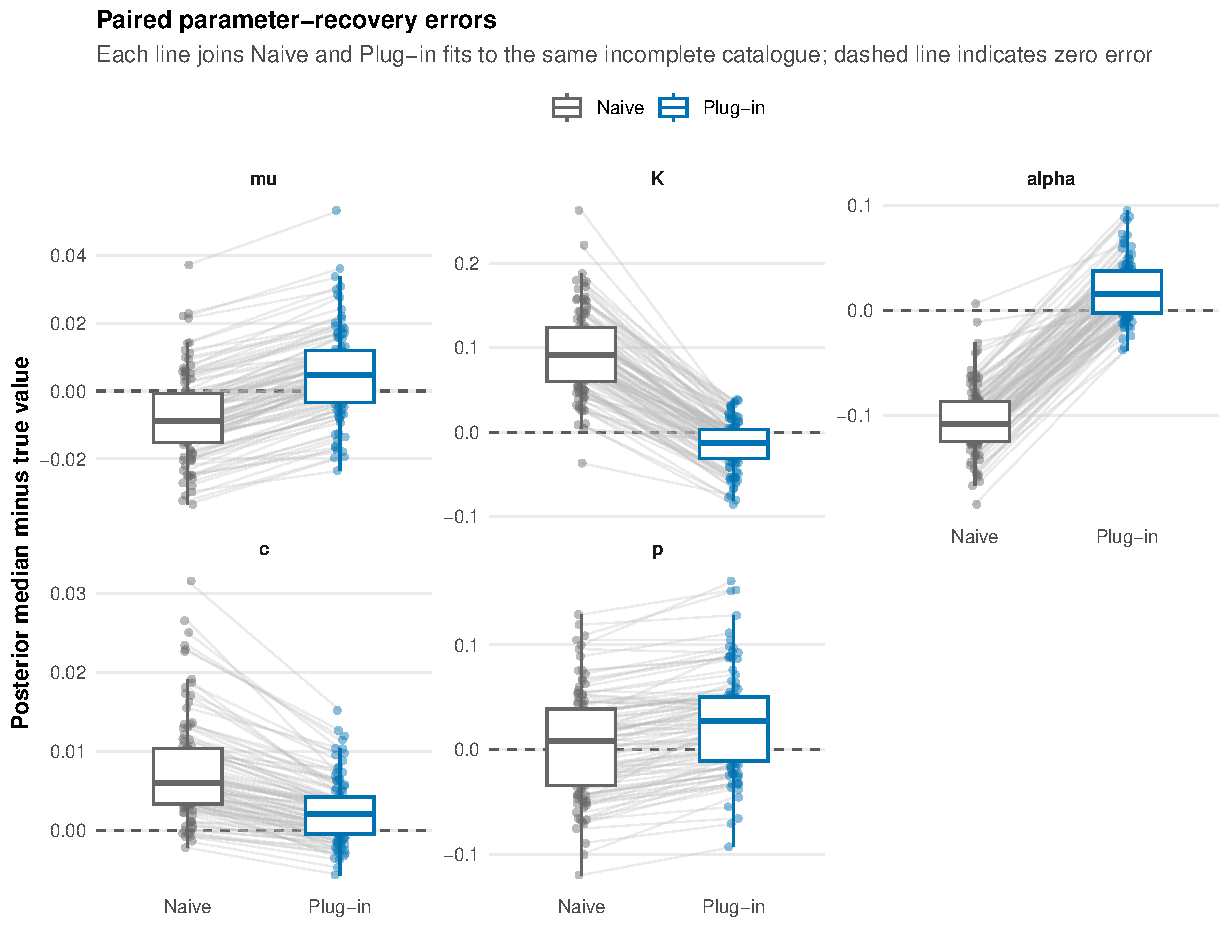
\includegraphics[width=0.80\textwidth]
  {../results/submission_v1/figures/thesis/03_synthetic_parameter_recovery.pdf}
  \caption{Paired parameter-recovery errors across 100 simulated incomplete
  catalogues. Points and boxplots show posterior-median estimation errors,
  defined as the posterior median minus the true value. Each grey line joins
  the Naive and Plug-in fits to the same catalogue, and the dashed horizontal
  line indicates zero error.}
  \label{fig:synthetic_parameter_recovery}
\end{figure}

The improvement was not uniform across all ETAS parameters. Plug-in reduced
the RMSE for \(\mu\) only slightly, from 0.0148 to 0.0143, and increased the
RMSE for \(p\) from 0.0510 to 0.0555. The catalogue-specific completeness
estimates had small signed biases, although their accuracy varied across
replicates: \(G\) had bias 0.0012 and RMSE 0.1348, while \(H\) had bias
0.0257 and RMSE 0.1270. Thus, the strongest recovery gains were concentrated
in \(K\), \(\alpha\), and \(c\), rather than occurring uniformly across the
full parameter vector.

The same pattern appeared in credible-interval calibration. Under Naive ETAS,
the empirical coverages of nominal 95\% credible intervals were 0.29 for
\(K\), 0.04 for \(\alpha\), and 0.69 for \(c\). These values show that the
Naive intervals frequently failed to contain the true triggering parameters.
Plug-in increased the corresponding coverages to 0.90, 0.90, and 0.92.
The correction therefore improved both posterior point estimation and the
repeated-sampling reliability of posterior uncertainty for these parameters
(Figure~\ref{fig:synthetic_coverage}).

\begin{figure}[htbp]
  \centering
  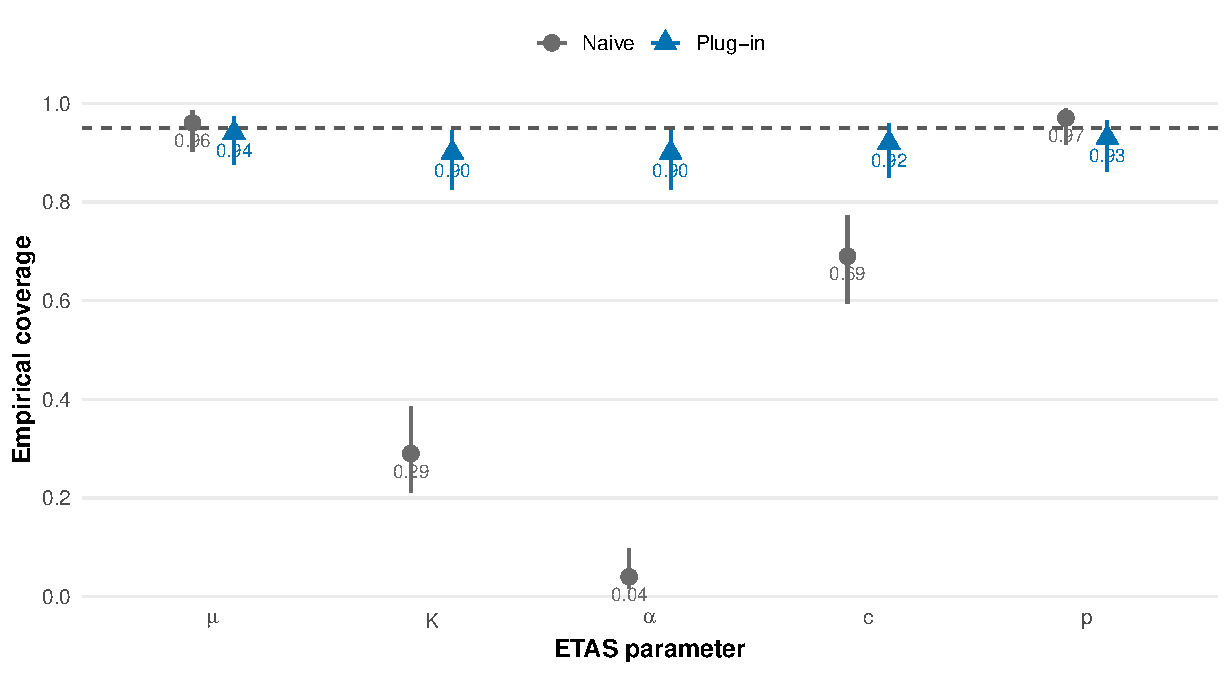
\includegraphics[width=0.80\textwidth]
  {../results/submission_v1/figures/thesis/04_synthetic_empirical_coverage.pdf}
  \caption{Empirical coverage of nominal 95\% credible intervals across 100
  simulated incomplete catalogues. Vertical intervals are 95\% Wilson
  intervals for the empirical coverage proportions, and the dashed horizontal
  line indicates the nominal coverage level of 0.95.}
  \label{fig:synthetic_coverage}
\end{figure}

The improvement in calibration was nevertheless incomplete. The 95\% Wilson
intervals for the Plug-in coverage estimates of \(K\) and \(\alpha\) were
both approximately \((0.826,0.945)\), leaving the nominal value of 0.95 just
outside their upper endpoints. Coverage for \(c\) was 0.92, with a Wilson
interval of approximately \((0.850,0.959)\), which included 0.95. Plug-in
therefore substantially reduced the severe undercoverage observed under Naive
ETAS, but did not achieve nominal empirical coverage for every triggering
parameter.

\subsection{Ridgecrest forecast performance}
\label{subsec:ridgecrest_forecast}

The frozen Ridgecrest catalogue contained 811 training-history events through
day 1 after the \(M7.1\) mainshock and 224 held-out events over days 1--10.
Fitting the single-mainshock completeness model to the training data gave
\((\widehat G,\widehat H)=(5.575,0.792)\). The fitted completeness threshold
returned to the baseline magnitude \(m_0=2.95\) approximately 0.016 days, or
23 minutes, after the mainshock
(Figure~\ref{fig:ridgecrest_completeness}).

\begin{figure}[htbp]
  \centering
  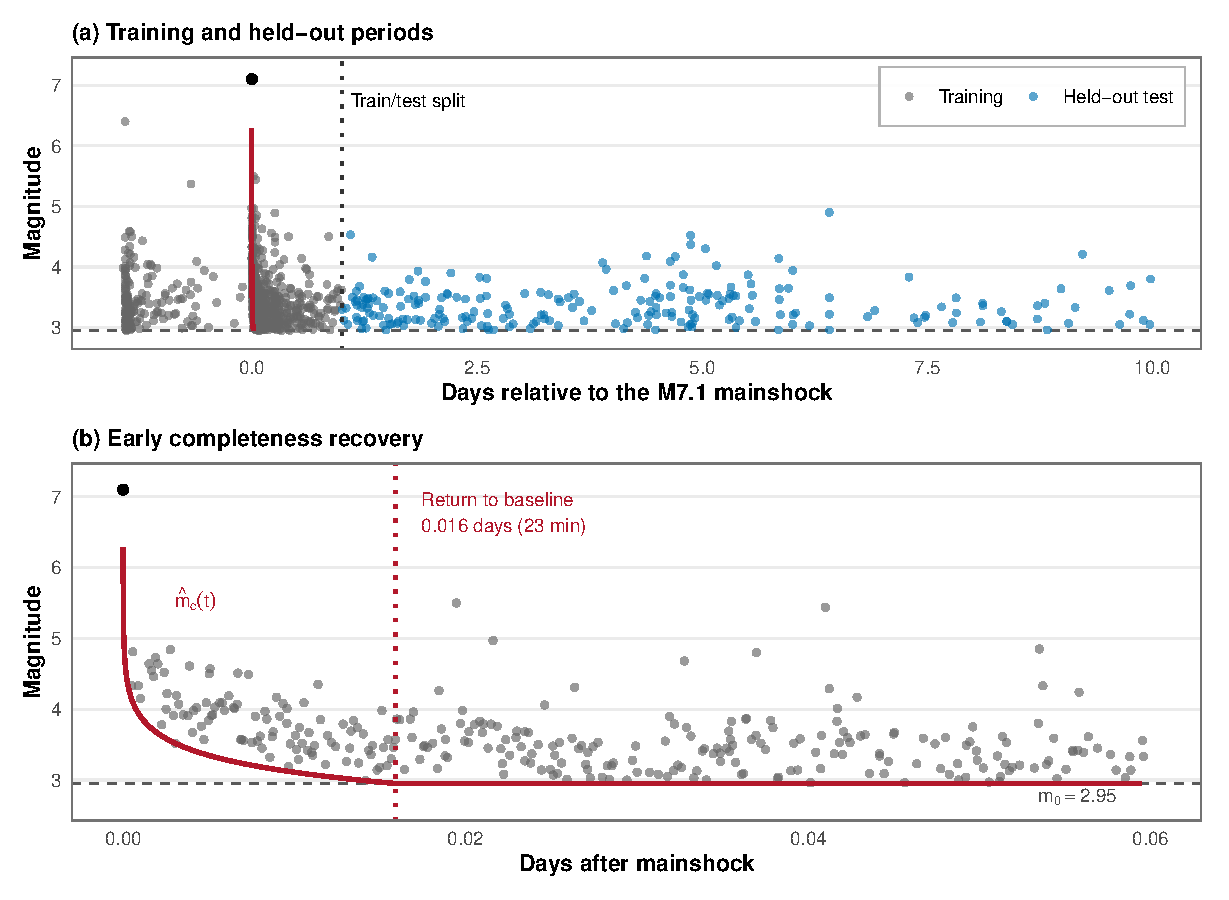
\includegraphics[width=0.80\textwidth]
  {../results/submission_v1/figures/thesis/05_ridgecrest_catalogue_completeness.pdf}
  \caption{Ridgecrest catalogue and fitted single-mainshock completeness
  threshold. Panel (a) shows the training and held-out periods, and panel (b)
  enlarges the early post-mainshock period used to estimate the completeness
  recovery.}
  \label{fig:ridgecrest_completeness}
\end{figure}

Both ETAS fits satisfied the pre-specified convergence criteria, with a
maximum \(\widehat R\) of 1.002 and a minimum effective sample size of 2,578.
Plug-in ETAS achieved a temporal log predictive density of 2.4293 per held-out
event, compared with 2.4036 under Naive ETAS. This corresponds to an
information gain of 0.0257 per event in favour of Plug-in. The associated
Monte Carlo interval was \((0.0241,0.0276)\), although this interval
quantifies posterior integration error for the fixed test catalogue rather
than variation across earthquake sequences.

The observed test-period count was 224. The posterior predictive median was
174 under Naive ETAS and 257.5 under Plug-in ETAS, making the Plug-in median
closer to the observed total. However, the Plug-in 95\% posterior predictive
interval was wider, increasing from \((71,741)\) under Naive ETAS to
\((146,1259)\). Its overflow probability was also higher, at 1.7\% compared
with 0.5\% under Naive ETAS. This greater upper-tail instability was
consistent with the posterior probability \(P(n\geq1)\), which increased from
0.019 under Naive ETAS to 0.838 under Plug-in ETAS.

The Ridgecrest case study therefore provides mixed predictive evidence. The
Plug-in correction improved temporal predictive density and produced a central
count prediction closer to the observation, but it also increased predictive
dispersion and upper-tail instability. These results do not establish broad
predictive superiority, but illustrate the predictive consequences of the
posterior changes identified in the synthetic experiment.

\clearpage
\section{Discussion}\label{sec:discussion}

\subsection{Main findings}

This study evaluated whether a Plug-in time-varying completeness correction
improves Bayesian ETAS inference under short-term catalogue incompleteness.
The repeated-simulation experiment showed substantial improvements for the
triggering parameters \(K\), \(\alpha\), and \(c\). Relative to Naive ETAS,
the Plug-in model reduced their RMSEs by 69.8\%, 68.4\%, and 53.0\%,
respectively. The paired comparisons showed that these gains occurred across
most catalogues rather than being driven by a few unusually poor Naive fits.

The correction also improved the repeated-sampling calibration of Bayesian
uncertainty. Naive 95\% credible intervals covered the true values of
\(K\), \(\alpha\), and \(c\) in only 29\%, 4\%, and 69\% of catalogues.
The corresponding Plug-in coverages were 90\%, 90\%, and 92\%. The benefits
were nevertheless parameter-specific: recovery of \(\mu\) changed little,
the RMSE for \(p\) increased slightly, and nominal coverage was not fully
restored for \(K\) and \(\alpha\).

The Ridgecrest case study provided similarly qualified evidence. Plug-in ETAS
assigned greater temporal predictive density to the fixed test catalogue and
produced a count median closer to the observed total. However, its predictive
count distribution was wider and its upper tail was less stable. Modelling
time-varying completeness therefore improved important aspects of inference
and prediction, but did not eliminate all consequences of missing events.

\subsection{Interpretation of the simulation results}

The Naive model treats the incomplete catalogue as complete above \(m_0\).
Immediately after the simulated mainshock, the underlying event rate is high
but the elevated detection threshold removes many small earthquakes. Naive
ETAS must explain the reduced number of recorded early aftershocks through the
seismicity model rather than through an observation process. This was most
evident in the overestimation of \(K\), underestimation of \(\alpha\), and
overestimation of \(c\).

These biases should be interpreted jointly. The parameters \(K\) and
\(\alpha\) control the number of triggered earthquakes and its dependence on
parent magnitude, while \(c\) controls the concentration of triggering at
short elapsed times. Different combinations can partly compensate for one
another when reproducing the incomplete observed catalogue. The Plug-in
likelihood reduces this distortion by allowing the early fall in recorded
events to be attributed partly to reduced detectability. Its strong paired
improvements for \(K\), \(\alpha\), and \(c\) indicate that this separation
was effective in most replicates.

The limited change in \(\mu\) is plausible because the background rate is
informed by the full catalogue, whereas incompleteness is concentrated in a
short post-mainshock period. The lack of improvement for \(p\) suggests that
the correction does not resolve every trade-off in the temporal kernel.
Correcting the earliest recorded rate may shift posterior dependence between
\(c\) and \(p\), so the results support parameter-specific rather than
universal claims about the correction.

\subsection{Remaining undercoverage}

Although Plug-in ETAS greatly reduced undercoverage, coverage for \(K\) and
\(\alpha\) remained at 0.90. Their Wilson intervals placed 0.95 just outside
the upper endpoint, so the discrepancy is not readily attributed to Monte
Carlo variation alone. One possible explanation is the Plug-in treatment of
the completeness parameters. The values of \(G\) and \(H\) were estimated
for each catalogue and then held fixed during ETAS inference. Their estimates
varied across replicates, but this uncertainty was not propagated into the
ETAS posterior and may have produced intervals that were too concentrated.

A second possible explanation is the observed-history approximation. The
correction adjusts the expected rate of detected events but does not restore
undetected earthquakes to the triggering history. If an undetected earthquake
triggers a later recorded event, the fitted model must explain that event using
the background rate or previously recorded parents. This structural loss of
triggering information remains even when the detectable fraction is correctly
specified. Finite catalogue size, posterior dependence, and the simplified
hard-threshold observation model may also contribute. The experiment does not
separately identify these mechanisms, so they should be regarded as plausible
explanations rather than established causes.

\subsection{Ridgecrest prediction}

For the fixed Ridgecrest test catalogue, Plug-in ETAS achieved an information
gain of 0.0257 per event. This indicates improved temporal predictive density
for this evaluation. The reported interval measures posterior Monte Carlo
integration error, however, and not variation across alternative earthquake
sequences or forecast windows. It therefore does not establish general
forecasting superiority.

The event-count results reinforce this qualification. The Plug-in median was
closer to the observed count, but its 95\% posterior predictive interval was
substantially wider. Its overflow probability and posterior probability of a
supercritical branching ratio were also higher. A central prediction closer
to the observation is desirable, but it must be considered together with the
dispersion and stability of the full predictive distribution. Evaluation over
additional earthquake sequences and prospectively specified test windows is
needed to determine whether the temporal gain persists and whether the heavy
upper tail is systematic.

\subsection{Relation to previous work}

The simulation findings are consistent with evidence that short-term
incompleteness can distort ETAS inference \citep{seif2017,naylor2023} and that
a time-dependent correction can move fitted posteriors closer to generating
values \citep{kamranzad2025}. The present study extends this evidence by
examining repeated-sampling coverage across 100 paired catalogues. Improved
posterior location and reliable interval calibration are distinct properties:
the Plug-in model substantially improved both, but did not attain nominal
coverage for every parameter.

The correction is comparatively straightforward to incorporate into Bayesian
ETAS fitting, but it is not a joint model of the complete latent catalogue.
Self-consistent approaches such as PETAI estimate detection and ETAS
components together \citep{mizrahi2021}. No direct comparison with those
methods was performed here, so the present results do not establish relative
superiority.

\subsection{Limitations and future work}

Several limitations constrain generalisation. First, the analysis used a
temporal rather than a spatio-temporal ETAS model. Second, the synthetic study
used a hard detection threshold following one seeded mainshock, whereas real
detection may vary gradually and multiple large earthquakes may generate
overlapping periods of incompleteness. Third, \(G\) and \(H\) were fixed
during ETAS inference. Fourth, the model did not infer latent undetected
earthquakes or their triggering contributions.

Empirical coverage was estimated from 100 catalogues under one generating
configuration. Further scenarios are required to assess sensitivity to the
severity and duration of incompleteness, catalogue length, productivity, and
prior specification. The real-data analysis was also limited to one sequence
and one held-out period. Future work could evaluate multiple sequences, use a
probabilistic detection model, and jointly infer completeness parameters,
ETAS parameters, and latent missing events.

\subsection{Conclusion}

Short-term catalogue incompleteness can distort both ETAS parameter estimates
and the apparent uncertainty of Bayesian inference. The Plug-in correction
substantially improved recovery and credible-interval coverage for
\(K\), \(\alpha\), and \(c\), but its benefits were not uniform and nominal
coverage was not fully restored. In Ridgecrest, it improved temporal
predictive density and the central count prediction while increasing
predictive dispersion and upper-tail instability. Accounting for
time-varying detectability is therefore important, but an observed-history
correction cannot fully recover information lost through undetected events.

\clearpage
\section{Reproducibility and data availability}

The simulation settings, priors, MCMC configuration, convergence criteria,
and ordered analysis scripts are provided with the dissertation code. The
repository also contains machine-readable summaries of the reported results,
software-version records, and checksums for the analysis code and frozen
catalogues. The Ridgecrest source catalogue was obtained from the USGS ComCat
service and frozen before model fitting. Its query parameters, selection
criteria, download date, and checksum are documented in the accompanying data
README. The compact submission contains the CSV summaries used for the tables
and numerical claims; regeneratable catalogues, preliminary fits, and large
posterior-draw objects are omitted and can be recreated by the ordered
workflow described in the repository README.

%=========================================================
%
%
%
% Students should not edit below here
%
%
%
%=========================================================

%=========================================================
%% Create bibliography
%
% References: modify the file refs.bib
%=========================================================

\clearpage
\pagenumbering{arabic}
\renewcommand*{\thepage}{References | Page \arabic{page}}

\bibliographystyle{apalike}
\bibliography{refs}

\end{document}
